\documentclass[conference]{IEEEtran}
\usepackage[utf8]{inputenc}
\usepackage[serbian]{babel}
\usepackage{graphicx}
\usepackage{float}
\usepackage{geometry}
\usepackage{amsmath}
\usepackage{amsfonts}
\usepackage{amssymb}
\usepackage{hyperref}
\usepackage{listings}
\usepackage{xcolor}

\geometry{margin=2cm}

\title{Veb platforma za testiranje znanja zasnovana na teoriji prostora znanja}

\author{\IEEEauthorblockN{Luka Đorđević - djordjevic.r218.2024@uns.ac.rs}
\IEEEauthorblockN{Marko Janošević - janosevic.r216.2024@uns.ac.rs}
\IEEEauthorblockA{\textit{Softversko Inženjerstvo i Informacione Tehnologije} \\
\textit{Univerzitet u Novom Sadu, Fakultet tehničkih nauka}\\
Novi Sad, Srbija \\
}}

\renewcommand{\thesection}{\Roman{section}}

\begin{document}

\maketitle

\section{Problem i motivacija}

Teorija prostora znanja (Knowledge Space Theory - KST) predstavlja matematički pristup modelovanju i analizi studentskog znanja pomoću strukturiranih grafova i adaptivnog testiranja. U savremenom obrazovnom sistemu, tradicionalni pristupi testiranju često ne pružaju dovoljno dubok uvid u strukturu znanja učenika, što ograničava mogućnosti za personalizovanu nastavu i otežava identifikaciju konkretnih oblasti koje zahtevaju dodatnu pažnju \cite{falmagne2006}.

Jedan od ključnih problema u ovom kontekstu jeste nedostatak centralizovane platforme koja bi omogućila nastavnicima da lako definišu prostor znanja, kreiraju testove u skladu sa tim prostorom i analiziraju studentske odgovore kroz interaktivnu vizualizaciju grafa znanja. Postojeći sistemi uglavnom ne podržavaju adaptivno testiranje, pri čemu se redosled pitanja prilagođava prethodnim odgovorima i očekivanoj strukturi znanja. Takođe, često izostaje i mogućnost upoređivanja očekivanog i stvarnog prostora znanja \cite{doignon1999}.

Predloženi sistem za testiranje znanja ima za cilj da odgovori na ove izazove kroz sledeće funkcionalnosti:

\begin{itemize}
  \item \textbf{Kreiranje grafa znanja} – Očekivani prostor znanja se modeluje kao usmeren graf u kojem čvorovi predstavljaju ključne teme, pojmove ili veštine, dok ivice opisuju zavisnosti između njih. Na taj način, nastavnici mogu intuitivno prikazati koje se oblasti nadovezuju jedna na drugu.
  
  \item \textbf{Adaptivno testiranje} – Redosled i izbor pitanja se dinamički prilagođavaju učenikovim prethodnim odgovorima i strukturi grafa. Ovo omogućava preciznije ispitivanje znanja, bez nepotrebnog ponavljanja poznatih oblasti.
  
  \item \textbf{Analiza rezultata i vizuelizacija} – Na osnovu tačnih i netačnih odgovora, sistem generiše stvarni prostor znanja svakog učenika, koji se zatim upoređuje sa očekivanim grafom. Vizuelna analiza pomaže i nastavnicima i učenicima da brzo uoče koje oblasti su savladane, a koje zahtevaju dodatno učenje.
  
  \item \textbf{Standardizovani izvoz testova} – Korišćenjem IMS QTI formata, testovi se mogu razmenjivati i koristiti u drugim platformama, čime se obezbeđuje interoperabilnost i skalabilnost rešenja.
\end{itemize}

Na ovaj način, platforma podržava kompletan obrazovni ciklus, od nastavnika koji definišu prostor znanja i prate napredak učenika, do studenata koji rešavaju testove i dobijaju personalizovane povratne informacije.



\section{TEORIJSKE OSNOVE}

\subsection{Teorija prostora znanja}

Teorija prostora znanja predstavlja matematički pristup modelovanju strukture znanja kroz koncepte iz teorije grafova i kombinatorike \cite{doignon1999}. Osnovna ideja je da se znanje modelira kao prostor stanja gde svako stanje predstavlja skup tema koje učenik poznaje. Graf znanja definiše zavisnosti između tema - ako učenik poznaje temu A, onda verovatno poznaje i temu B koja zavisi od A.

Ključni koncepti teorije prostora znanja uključuju:
\begin{itemize}
\item \textbf{Čvorovi grafa} - Predstavljaju pojedinačne teme ili koncepte
\item \textbf{Ivice grafa} - Definišu zavisnosti između tema
\item \textbf{Stanje znanja} - Skup tema koje učenik poznaje
\item \textbf{Prostor znanja} - Kolekcija svih mogućih stanja znanja
\end{itemize}

Teorija prostora znanja zasniva se na pretpostavci da znanje nije linearno, već da postoje hijerarhijske zavisnosti između različitih koncepata. Na primer, učenik ne može da razume kompleksne matematičke koncepte bez poznavanja osnovnih matematičkih operacija. Ova hijerarhija se modeluje kroz usmerene grafove gde čvorovi predstavljaju pojedinačne koncepte, a ivice označavaju preduslove za učenje.

Matematički, prostor znanja se definiše kao par $(Q, \mathcal{K})$ gde je $Q$ skup svih mogućih pitanja ili koncepata, a $\mathcal{K}$ je kolekcija podskupova od $Q$ koji predstavljaju moguća stanja znanja. Svako stanje znanja $K \in \mathcal{K}$ predstavlja skup koncepata koje učenik poznaje u određenom trenutku.

Adaptivno testiranje u okviru teorije prostora znanja omogućava dinamičko prilagođavanje redosleda pitanja na osnovu trenutnog stanja znanja učenika. Algoritam za adaptivno testiranje koristi informacije o očekivanom prostoru znanja da bi odredio koje pitanje je najprikladnije za postavljanje u sledećem koraku. Ovo se postiže kroz analizu zavisnosti između koncepata i trenutnog stanja znanja učenika.

Generisanje stvarnog prostora znanja na osnovu studentskih rezultata predstavlja ključni aspekt teorije. Na osnovu odgovora na pitanja, sistem može da zaključi koje koncepte učenik poznaje, a koje ne. Ova informacija se koristi za kreiranje personalizovanog grafa znanja koji reflektuje stvarno stanje znanja učenika. Za generisanje stvarnog prostora znanja koristi se ITA (Item Tree Analysis) algoritam \cite{vanleeuwen2006}, koji predstavlja statističku metodu za analizu hijerarhijskih zavisnosti između pitanja. ITA algoritam analizira frekvenciju tačnih odgovora na pitanja i identifikuje potencijalne zavisnosti između njih. Algoritam koristi koncepte iz teorije grafova da bi konstruisao stablo zavisnosti između pitanja, gde čvorovi predstavljaju pitanja, a ivice označavaju statističke zavisnosti. ITA algoritam je posebno koristan jer omogućava automatsko otkrivanje strukture znanja na osnovu empirijskih podataka, što omogućava validaciju očekivanog prostora znanja i identifikaciju potencijalnih grešaka u definisanju zavisnosti između koncepata.


\subsection{Tehnologije}

Platforma objedinjuje brojne moderne tehnologije koje pružaju skalabilnost, sigurnost i pouzdanost.

\subsubsection{Backend}
Backend aplikacija implementirana je u Python Flask radnom okviru. Flask predstavlja fleksibilan radni okvir koji omogućava brz razvoj REST API-ja \cite{flask2020}. Odabran je zbog svoje jednostavnosti, dobre dokumentacije i bogatog ekosistema biblioteka za rad sa bazama podataka i autentifikacijom.

\subsubsection{Frontend}
Frontend aplikacija implementirana je upotrebom React biblioteke u okviru programskog jezika TypeScript. React predstavlja fleksibilnu biblioteku za izgradnju korisničkog interfejsa \cite{react2020} sa komponentnim pristupom koji omogućava efikasno upravljanje stanjem aplikacije. TypeScript pruža statičku tipizaciju koja smanjuje greške u razvoju.

\subsubsection{Baza podataka}
Za perzistenciju podataka korišćena je PostgreSQL relaciona baza podataka \cite{postgresql2020}. PostgreSQL je odabran zbog svoje pouzdanosti, podrške za kompleksne upite i dobre integracije sa Python ekosistemom. Baza čuva sve podatke o korisnicima, testovima, pitanjima, rezultatima i grafovima znanja.

\subsubsection{Graf vizualizacija}
Za vizualizaciju grafova znanja korišćena je biblioteka D3.js \cite{d3js2020}. D3.js omogućava kreiranje interaktivnih vizuelizacija podataka i pruža napredne mogućnosti za manipulaciju grafovima, uključujući animacije, interaktivnost i dinamičko ažuriranje.

\section{SRODNA ISTRAŽIVANJA}

Istraživanja u oblasti teorije prostora znanja i adaptivnog testiranja imaju dugu istoriju i obuhvataju različite pristupe i aplikacije. Prvi radovi na teoriji prostora znanja potiču iz 1980-ih godina, kada su Doignon i Falmagne uveli matematički formalizam za modelovanje strukture znanja \cite{doignon1999}. Od tada je ova teorija našla primenu u različitim oblastima obrazovanja, od osnovnog školstva do visokog obrazovanja.

Jedan od ključnih radova u ovoj oblasti je ALEKS (Assessment and Learning in Knowledge Spaces) sistem \cite{aleks2009}, koji predstavlja komercijalnu implementaciju teorije prostora znanja. ALEKS sistem koristi adaptivno testiranje za procenu studentskog znanja u matematičkim disciplinama i pruža personalizovane planove učenja. Sistem je pokazao značajne rezultate u poboljšanju studentskog učenja, posebno u oblasti matematike i nauke.

U oblasti algoritama za analizu prostora znanja, ITA (Item Tree Analysis) algoritam predstavlja jedan od najznačajnijih doprinosa \cite{vanleeuwen2006}. Ovaj algoritam omogućava automatsko otkrivanje hijerarhijskih zavisnosti između pitanja na osnovu empirijskih podataka, što je posebno korisno za validaciju ekspertno definisanih prostora znanja. ITA algoritam je primenjen u različitim kontekstima, od psihologije do obrazovanja, i pokazao je visoku pouzdanost u identifikaciji strukture znanja.

Adaptivno testiranje zasnovano na teoriji prostora znanja predstavlja aktivnu oblast istraživanja. Različiti algoritmi za adaptivno testiranje su razvijeni, uključujući algoritme zasnovane na teoriji odziva na pitanja (Item Response Theory) i teoriji prostora znanja. Komparativne studije su pokazale da pristupi zasnovani na teoriji prostora znanja mogu biti efikasniji za procenu specifičnih koncepata i identifikaciju nedostataka u znanju \cite{desmarais2012}.

Vizuelizacija prostora znanja predstavlja relativno novu oblast istraživanja. Različiti pristupi za vizuelizaciju grafova znanja su razvijeni, uključujući interaktivne grafove, dendrograme i mreže. Studije su pokazale da vizuelizacija može značajno poboljšati razumevanje strukture znanja kod nastavnika i studenata \cite{chen2014}.

U oblasti standardizacije testova, IMS QTI (Question and Test Interoperability) specifikacija predstavlja važan standard za razmenu testova između različitih obrazovnih sistema \cite{imsqti2012}. Ova specifikacija omogućava interoperabilnost između različitih platformi za testiranje i pruža standardizovan format za definisanje pitanja, odgovora i rezultata.

Komparativna analiza postojećih platformi za testiranje pokazuje da većina sistema ne podržava teoriju prostora znanja ili pruža ograničenu podršku za adaptivno testiranje. Postojeći sistemi često se fokusiraju na tradicionalne pristupe testiranju, što ograničava njihovu efikasnost za procenu kompleksnih struktura znanja.

\section{REŠENJE}

\subsection{Arhitektura sistema}

Platforma je dizajnirana kao web aplikacija sa klijent-server arhitekturom, organizovana u tri glavne komponente: frontend, backend i baza podataka. Svaka komponenta ima specifičnu ulogu u sistemu i komunicira sa ostalim komponentama kroz standardizovane interfejse.

\begin{figure}[H]
\centering
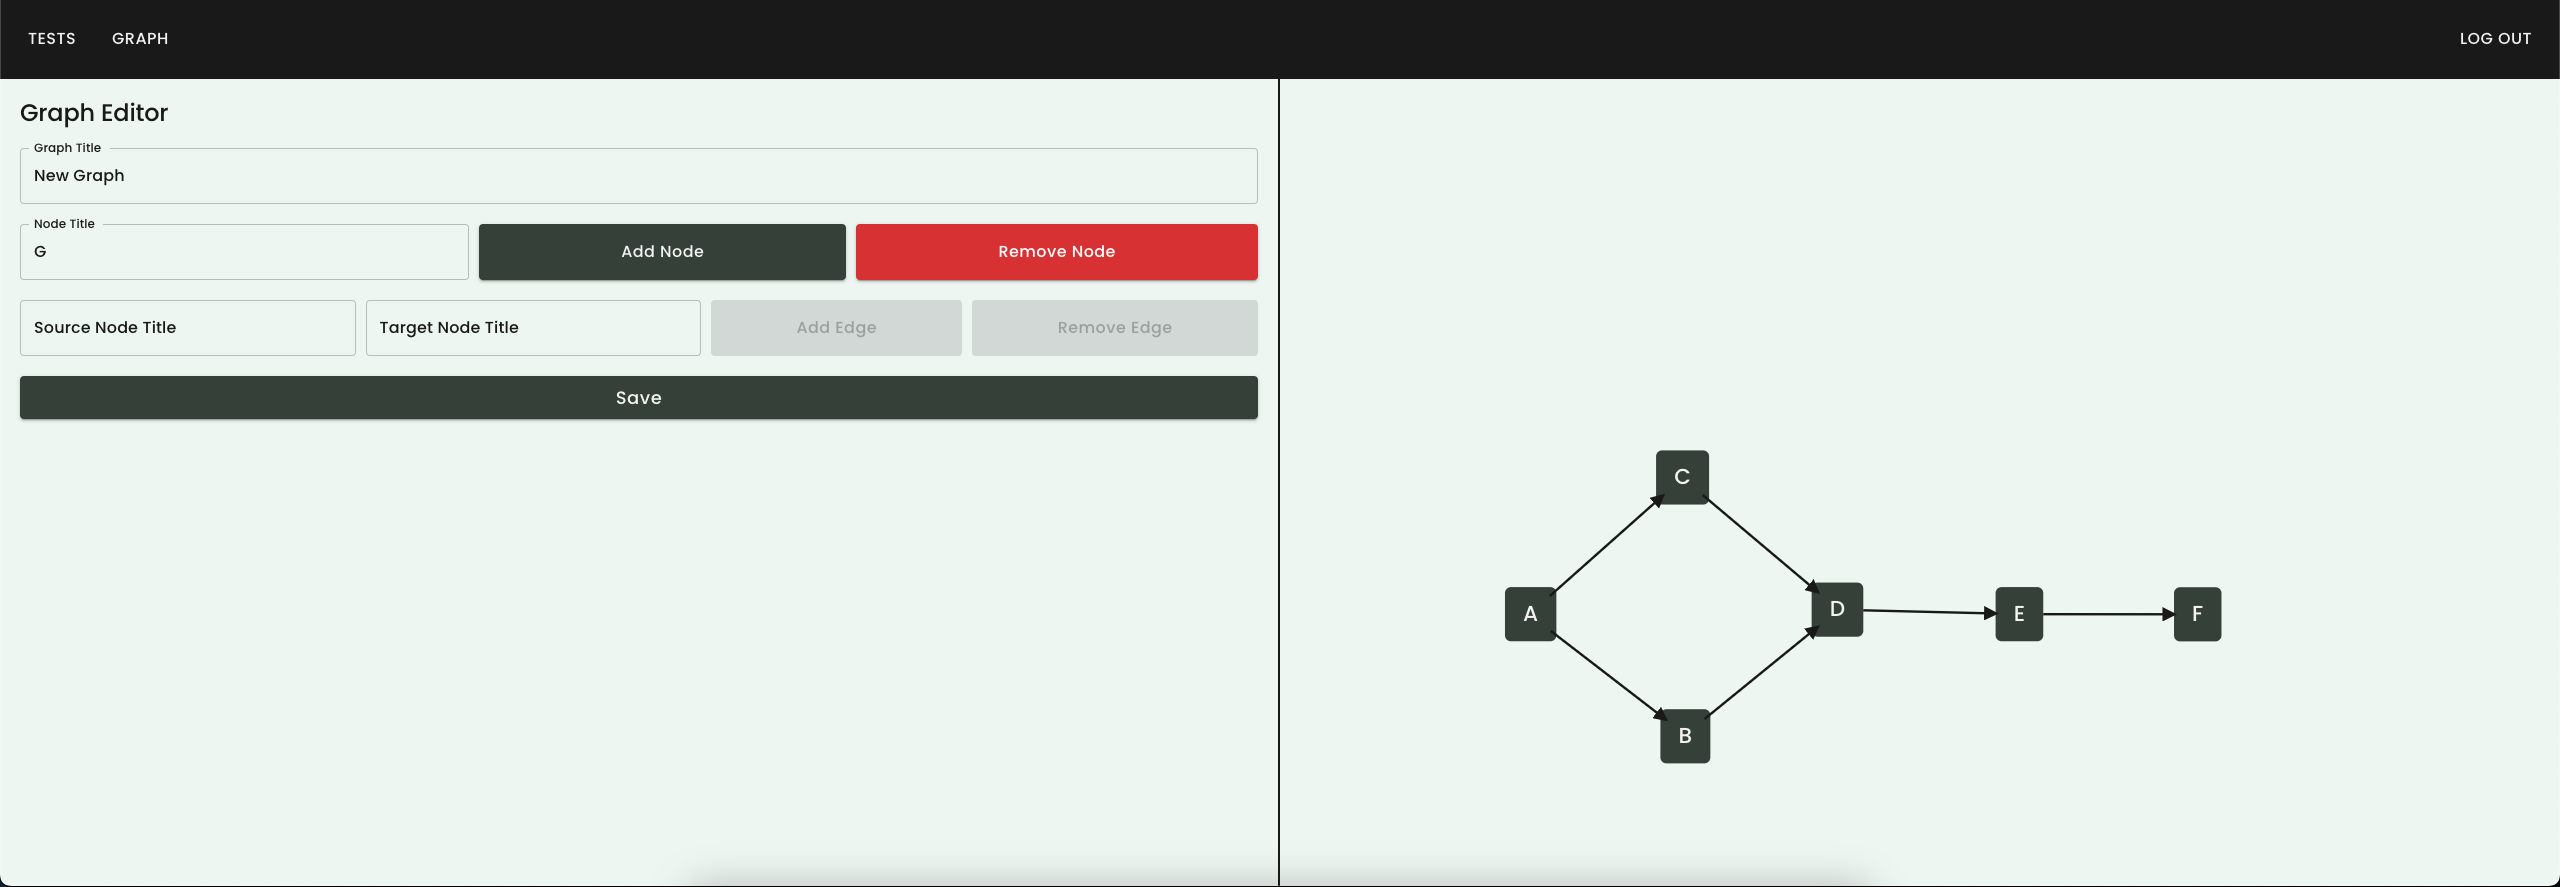
\includegraphics[width=0.8\columnwidth]{graph-create.png}
\caption{Arhitektura sistema}
\end{figure}

Frontend komponenta predstavlja korisnički interfejs platforme i izrađena je u React biblioteci uz upotrebu TypeScript programskog jezika. Komponenta je organizovana u modulnu strukturu gde svaki modul odgovara specifičnoj funkcionalnosti sistema. Glavni moduli uključuju autentifikaciju, kreiranje grafova, kreiranje testova, pregled rezultata i upoređivanje grafova. Frontend komponenta komunicira sa backend-om kroz REST API interfejs.

Backend komponenta predstavlja srž sistema i implementirana je u Python Flask radnom okviru. Organizovana je u tri glavna sloja: controller, service i repository. Controller sloj je zadužen za obradu HTTP zahteva, validaciju podataka i rutiranje. Service sloj sadrži biznis logiku sistema, uključujući algoritme za adaptivno testiranje i generisanje prostora znanja. Repository sloj omogućava komunikaciju sa bazom podataka kroz SQLAlchemy ORM.

Baza podataka je implementirana u PostgreSQL sistemu i organizovana u devet glavnih tabela. Tabele su dizajnirane da podržavaju sve funkcionalnosti platforme, uključujući upravljanje korisnicima, kreiranje testova, čuvanje rezultata i modelovanje grafova znanja. Relacije između tabela su definisane kroz strane ključeve koji omogućavaju integritet podataka.

\subsection{Funkcionalni opis}

Platforma omogućava kompletan tok rada od kreiranja grafova znanja do analize studentskih rezultata. Proces počinje kada nastavnik kreira graf znanja definisanjem čvorova (teme) i ivica (zavisnosti). Graf se dinamički vizualizuje u realnom vremenu, omogućavajući nastavniku da vidi strukturu znanja dok je kreira.

Nakon kreiranja grafa, nastavnik može da kreira test definisanjem pitanja i povezivanjem svakog pitanja sa odgovarajućim čvorom grafa. Sistem podržava različite tipove pitanja, uključujući pitanja sa višestrukim izborom. Svako pitanje može imati više odgovora, od kojih je jedan ili više tačnih.

\begin{figure*}[ht]
\centering
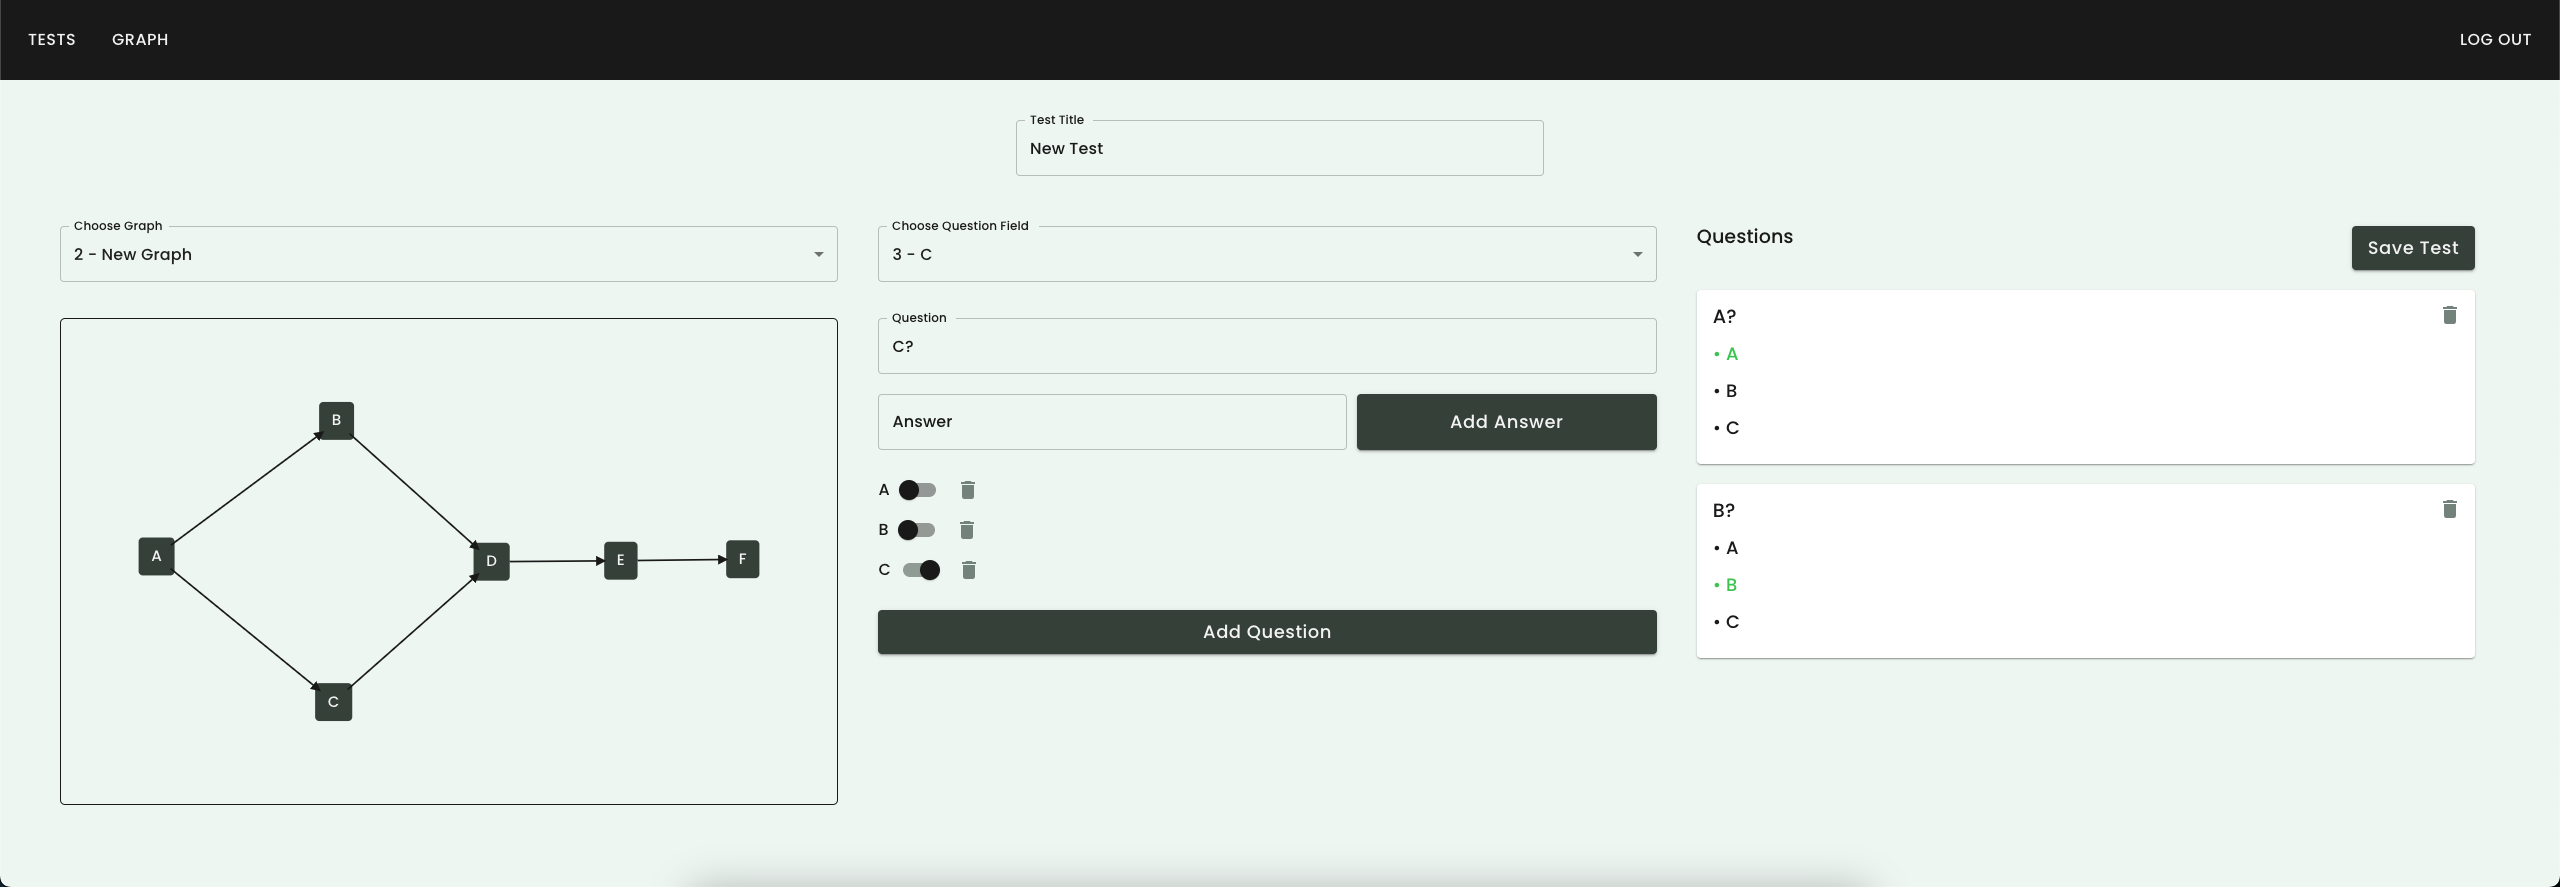
\includegraphics[width=1\textwidth]{test-create.png}
\caption{Kreiranje testova}
\label{fig:graf_programiranja}
\end{figure*}

Kada student započne test, sistem primenjuje BFS (Breadth First Search) nad grafom znanja koji je definisan za taj test kako bi formirao redosled pitanja. Graf modeluje relacije između koncepata, pa se pretragom po širini prvo posećuju čvorovi (pitanja) na minimalnoj udaljenosti od korena, odnosno osnovni koncepti, a zatim se prelazi na sve složenije nivoe.

Na osnovu odgovora, sistem može da zaključi koje koncepte studenti poznaju, a koje ne. Ova informacija se koristi za generisanje grafa znanja koji reflektuje stvarno stanje znanja studenata.

Nakon završetka testa, nastavnik može da analizira rezultate kroz različite vizuelizacije. Sistem omogućava poređenje očekivanog i stvarnog prostora znanja i identifikaciju nedostataka u znanju. Rezultati se mogu eksportovati u IMS QTI format za kompatibilnost sa drugim obrazovnim sistemima.

\begin{figure}[H]
\centering
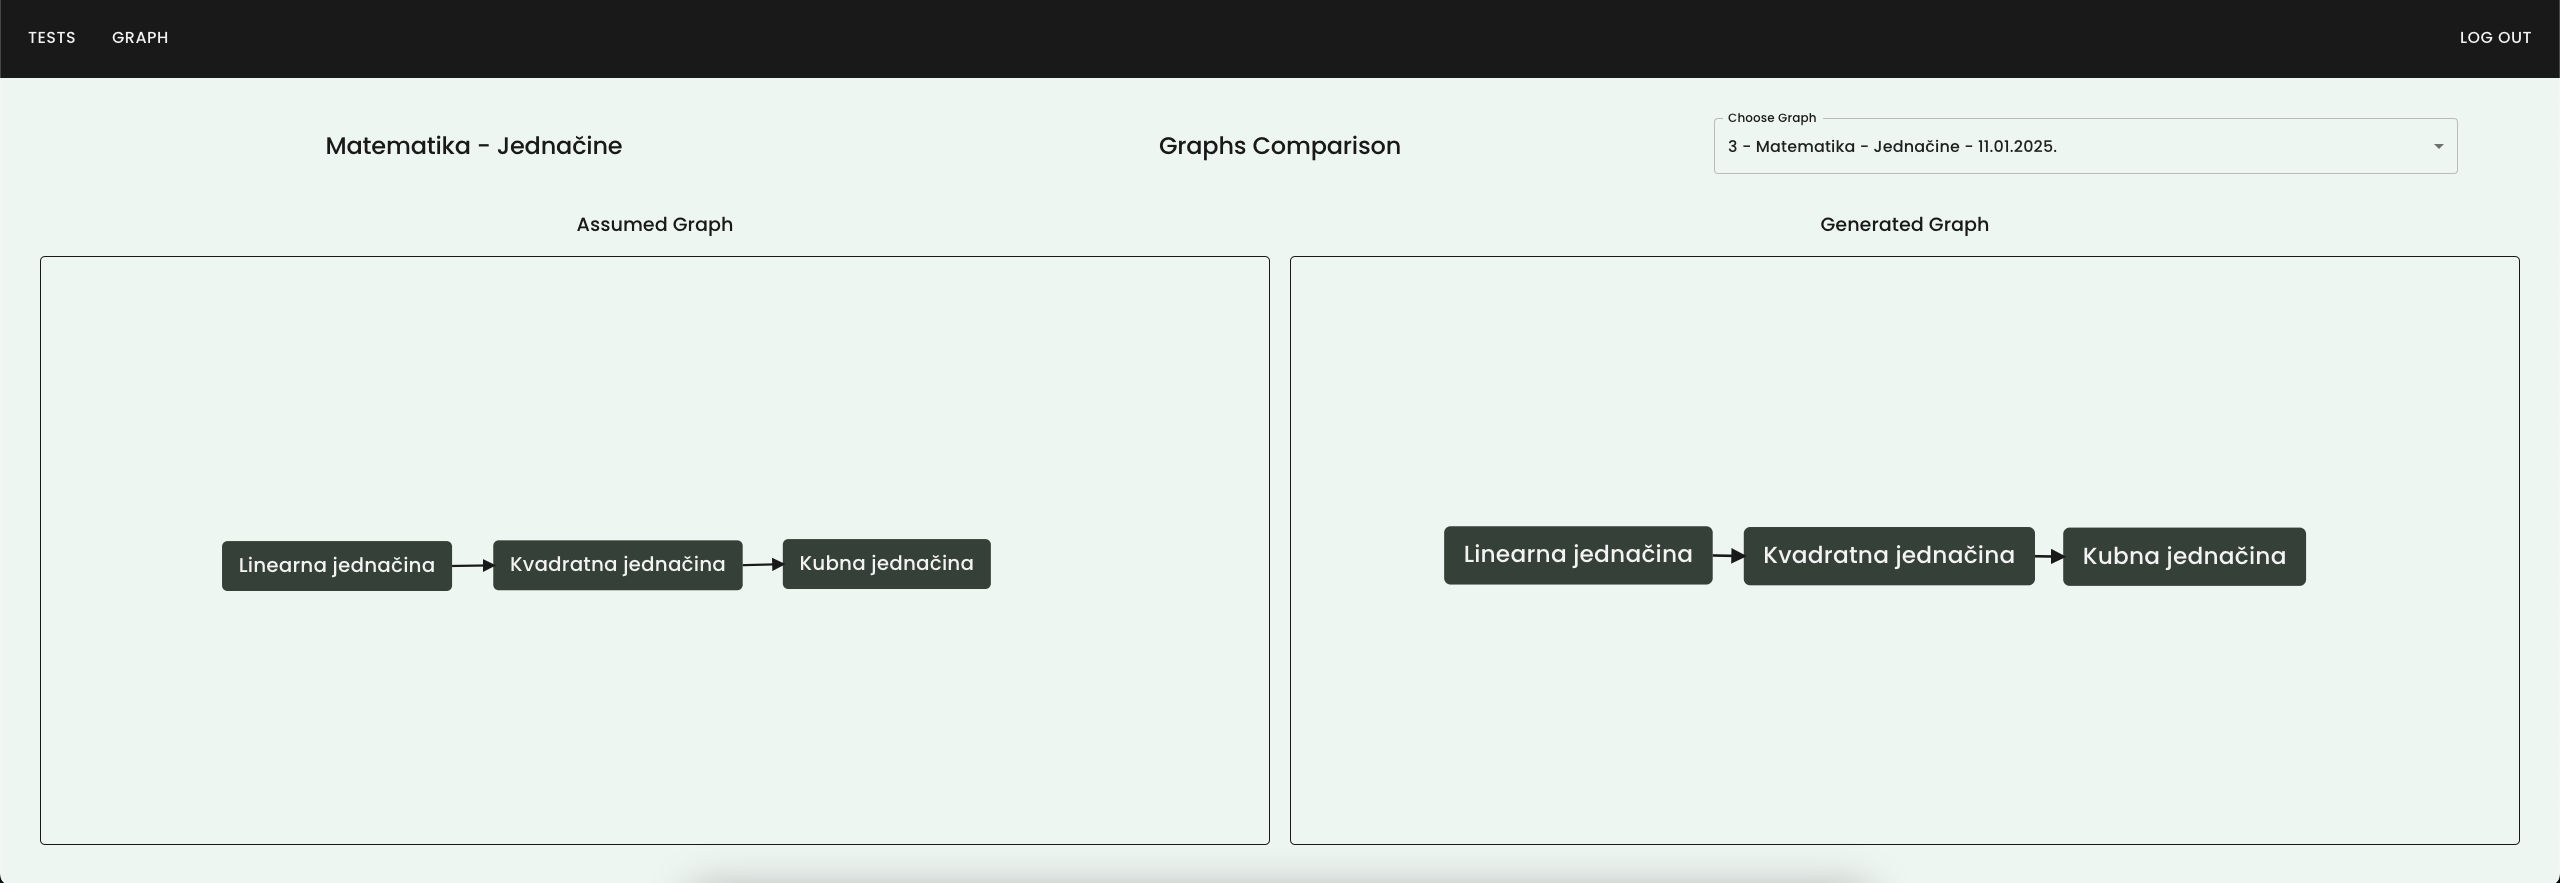
\includegraphics[width=0.8\columnwidth]{graphs-comparison.png}
\caption{Upoređivanje stvarnog i očekivanog prostora znanja}
\end{figure}

Platforma takođe podržava napredne funkcionalnosti kao što su grupni pregled rezultata testa i generisanje grafa znanja na osnovu svih rezultata u izabranom vremenskom periodu. Sve funkcionalnosti su dizajnirane da budu intuitivne i lake za korišćenje, omogućavajući nastavnicima da se fokusiraju na pedagoške aspekte umesto na tehničke detalje.

\section{DISKUSIJA}

Implementacija platforme za testiranje znanja zasnovana na teoriji prostora znanja pokazala je značajne prednosti u odnosu na tradicionalne pristupe testiranju. Ključni doprinosi platforme uključuju kreiranje testova zasnovanih na teoriji prostora znanja, adaptivno testiranje koje prilagođava redosled pitanja, vizualizaciju i upoređivanje očekivanog i stvarnog prostora znanja, te IMS QTI eksport za kompatibilnost sa drugim sistemima.

\subsection{Prednosti platforme}

Platforma pokazuje značajne prednosti u odnosu na tradicionalne sisteme za testiranje. Prva i najvažnija prednost je mogućnost vizuelnog kreiranja grafova znanja, što omogućava nastavnicima da jasno definišu hijerarhijske zavisnosti između koncepata. Ova funkcionalnost je posebno korisna za kompleksne predmete gde postoje jasne zavisnosti između tema, kao što su matematika, fizika ili programiranje.

Adaptivno testiranje predstavlja drugu ključnu prednost platforme. Umesto fiksnog redosleda pitanja, sistem dinamički prilagođava test na osnovu trenutnog stanja znanja studenata. Ovo omogućava efikasniju procenu znanja i smanjuje frustraciju studenata koji se suočavaju sa pitanjima za koja nisu spremni. Adaptivni pristup takođe omogućava bržu identifikaciju nedostataka u znanju i fokusiranje na područja koja zahtevaju dodatnu pažnju.

Vizualizacija rezultata predstavlja treću značajnu prednost. Mogućnost poređenja očekivanog i stvarnog prostora znanja omogućava nastavnicima da identifikuju greške u definisanju zavisnosti između koncepata i da poboljšaju strukturu nastave. Vizuelni prikaz takođe pomaže studentima da bolje razumeju svoje znanje i identifikuju područja za poboljšanje.

\subsection{Ograničenja i izazovi}

Uprkos prednostima, platforma ima određena ograničenja koja treba uzeti u obzir. 

Prvo ograničenje se odnosi na kompleksnost kreiranja grafova znanja. Za veće predmete sa mnogo tema, kreiranje detaljnog grafa može biti vremenski zahtevno i zahtevati značajnu ekspertizu nastavnika. Ovo ograničenje može se rešiti kroz razvoj naprednih alata za automatsko generisanje grafova na osnovu postojećih kurikuluma.

Drugo ograničenje se odnosi na validaciju grafova znanja. Ekspertno definisani grafovi mogu sadržati greške u definisanju zavisnosti između koncepata, što može uticati na efikasnost adaptivnog testiranja. ITA algoritam pomaže u identifikaciji ovih grešaka, ali potrebno je dodatno istraživanje u oblasti automatske validacije grafova.

Treće ograničenje se odnosi na skalabilnost platforme. Za veće institucije sa velikim brojem studenata i testova, potrebno je implementirati napredne tehnike optimizacije i distribuirane arhitekture. Trenutna implementacija je optimizovana za manje do srednje institucije.

\subsection{Komparacija sa postojećim rešenjima}

Komparacija sa postojećim platformama za testiranje pokazuje da ova platforma pruža jedinstvene funkcionalnosti koje nisu dostupne u većini komercijalnih rešenja. 
ALEKS sistem predstavlja najbliži komercijalni ekvivalent našoj platformi, ali je ograničen na matematičke discipline i ne pruža mogućnost kreiranja grafova znanja iz različitih oblasti. Naša platforma je dizajnirana da bude generička i primenjiva na različite discipline.

\section{ZAKLJUČAK}

Implementacija platforme za testiranje znanja zasnovana na teoriji prostora znanja uspešno rešava probleme tradicionalnog testiranja kroz adaptivni pristup i vizualizaciju strukture znanja. Rezultati implementacije pokazuju visoku korisnost i efikasnost sistema u odnosu na postojeća rešenja.

Implementacija ITA algoritma za generisanje stvarnog prostora znanja omogućila je automatsko otkrivanje strukture znanja na osnovu empirijskih podataka, što omogućava validaciju ekspertno definisanih prostora znanja i identifikaciju potencijalnih grešaka u definisanju zavisnosti između koncepata.

Budući rad treba da se fokusira na nekoliko ključnih oblasti. Prva oblast se odnosi na razvoj naprednih algoritama za automatsko generisanje grafova znanja na osnovu postojećih kurikuluma i nastavnih materijala. Ovo bi značajno smanjilo opterećenje nastavnika i omogućilo bržu implementaciju platforme.

Druga oblast se odnosi na implementaciju naprednih tehnika mašinskog učenja za poboljšanje adaptivnog testiranja. Algoritmi zasnovani na dubokom učenju mogu poboljšati preciznost procene studentskog znanja i omogućiti predviđanje budućeg napretka.

Treća oblast se odnosi na razvoj mobilnih aplikacija i integraciju sa postojećim sistemima za upravljanje učenjem (LMS). Ovo bi omogućilo širu primenu platforme u različitim obrazovnim kontekstima.

Četvrta oblast se odnosi na evaluaciju efikasnosti platforme kroz dugoročne studije u realnim obrazovnim okruženjima. Potrebno je sprovesti detaljne studije koje će meriti uticaj platforme na studentsko učenje i zadržavanje znanja.

Platforma predstavlja značajan korak napred u oblasti adaptivnog testiranja i vizuelizacije prostora znanja, pružajući temelje za buduća istraživanja u oblasti personalizovanog obrazovanja i analitike učenja.

\begin{thebibliography}{1}

\bibitem{falmagne2006}
J.~C. Falmagne and J.~P. Doignon,
\newblock ``Knowledge spaces and learning spaces,''
\newblock \emph{Mathematical Psychology}, vol.~50, no.~2, pp.~123--135, 2006.

\bibitem{doignon1999}
J.~P. Doignon and J.~C. Falmagne,
\newblock \emph{Knowledge Spaces},
\newblock Springer-Verlag, Berlin, 1999.

\bibitem{vanleeuwen2006}
M.~van der Linden and W.~J. van der Linden,
\newblock ``Item tree analysis,''
\newblock \emph{Applied Psychological Measurement}, vol.~30, no.~3, pp.~189--213, 2006.

\bibitem{aleks2009}
ALEKS Corporation,
\newblock ``Assessment and Learning in Knowledge Spaces,''
\newblock McGraw-Hill Education, 2009.

\bibitem{desmarais2012}
M.~C. Desmarais and R.~S. Baker,
\newblock ``A review of recent advances in learner and skill modeling in intelligent learning environments,''
\newblock \emph{User Modeling and User-Adapted Interaction}, vol.~22, no.~1-2, pp.~9--38, 2012.

\bibitem{chen2014}
C.~Chen and M.~Czerwinski,
\newblock ``Empirical evaluation of information visualizations: An introduction,''
\newblock \emph{International Journal of Human-Computer Studies}, vol.~53, no.~5, pp.~631--635, 2014.

\bibitem{imsqti2012}
IMS Global Learning Consortium,
\newblock ``IMS Question and Test Interoperability Specification,''
\newblock Version 2.2, 2012.

\bibitem{flask2020}
Flask Development Team,
\newblock ``Flask: A lightweight WSGI web application framework,''
\newblock \url{https://flask.palletsprojects.com/}, 2020.

\bibitem{react2020}
Facebook Inc.,
\newblock ``React: A JavaScript library for building user interfaces,''
\newblock \url{https://reactjs.org/}, 2020.

\bibitem{postgresql2020}
PostgreSQL Global Development Group,
\newblock ``PostgreSQL: The world's most advanced open source relational database,''
\newblock \url{https://www.postgresql.org/}, 2020.

\bibitem{d3js2020}
M.~Bostock,
\newblock ``D3.js: Data-Driven Documents,''
\newblock \url{https://d3js.org/}, 2020.

\end{thebibliography}

\end{document} 